\documentclass[11pt]{article}
\usepackage{amsmath,amssymb,amsthm, mathtools, tikz}
\usetikzlibrary{shapes}

\DeclareMathOperator*{\E}{\mathbb{E}}
\let\Pr\relax
\DeclareMathOperator*{\Pr}{\mathbb{P}}

\newcommand{\eps}{\varepsilon}
\newcommand{\inprod}[1]{\left\langle #1 \right\rangle}
\newcommand{\R}{\mathbb{R}}
\newcommand{\TODO}{TODO TODO TODO TODO \\}

\newcommand{\handout}[5]{
  \noindent
  \begin{center}
  \framebox{
    \vbox{
      \hbox to 5.78in { {\bf CS 224: Advanced Algorithms } \hfill #2 }
      \vspace{4mm}
      \hbox to 5.78in { {\Large \hfill #5  \hfill} }
      \vspace{2mm}
      \hbox to 5.78in { {\em #3 \hfill #4} }
    }
  }
  \end{center}
  \vspace*{4mm}
}

\newcommand{\lecture}[4]{\handout{#1}{#2}{#3}{Scribe: #4}{Lecture #1}}

\newtheorem{theorem}{Theorem}
\newtheorem{corollary}[theorem]{Corollary}
\newtheorem{lemma}[theorem]{Lemma}
\newtheorem{observation}[theorem]{Observation}
\newtheorem{proposition}[theorem]{Proposition}
\newtheorem{definition}[theorem]{Definition}
\newtheorem{claim}[theorem]{Claim}
\newtheorem{fact}[theorem]{Fact}
\newtheorem{assumption}[theorem]{Assumption}

% 1-inch margins, from fullpage.sty by H.Partl, Version 2, Dec. 15, 1988.
\topmargin 0pt
\advance \topmargin by -\headheight
\advance \topmargin by -\headsep
\textheight 8.9in
\oddsidemargin 0pt
\evensidemargin \oddsidemargin
\marginparwidth 0.5in
\textwidth 6.5in

\parindent 0in
\parskip 1.5ex

\begin{document}

\lecture{8 --- Feb 16, 2017}{Spring 2017}{Prof.\ Jelani Nelson}{Tiffany}

\section{Overview}

In the last lecture we covered the properties of splay trees, including amortized $O(\log n)$ time for operations, static finger, dynamic finger, and others. 

In this lecture we analyze splay trees, and begin discussion of online algorithms. 

\section{Splay Tree Analysis}

\subsection{Notation}
Define a weight function on nodes $w:\{nodes\}\to \R_{\ge 0}$. We will write our potential function in terms of $w$, and by taking different weight functions will allow us to prove different properties, such as amortized $O(\log n)$ operations and static optimality later on in this lecture. For now, think of $w(x) = 1$. 

Additionally, define 

\[s(x) \coloneqq \sum_{\substack{y\in x\text{ subtree}\\\text{including} x}}w(y)\]

and let the rank of a node $x$ be $r(x) \coloneqq \lg(s(x))$. It's not clear including a log here is well motivated, and indeed the original authors of the paper say as much.

The potential function on a particular state $S$ of the splay tree is
    \[\phi(S) \coloneqq \sum_{x \in T} r(x)\]
Additionally, let $W = \sum_{x\in T} w(x)$ be the size of the root.

\subsection{Analysis of splay(x) taking $O(\log n)$ time}

Set $w(x) = 1$. 
\begin{claim}
The amortized cost of splay(x) is \[\tilde{t}_{splay} \le 3\cdot(r(root) - r(x)) + 1 \le 3\log(n) + 1\]
since the root has weight $n$.
\end{claim}

\begin{claim}
Suppose we are doing one of the cases of (1) zig, (2) zig-zig, or (3)zig-zag. Then amortized cost of performing each of these operations is 
\begin{itemize}
    \item Case (1): $3(r'(x)-r(x))+1$ where $r'(x)$ is the rank of $x$ after the operation.
    \item Cases (2), (3): $3(r'(x) - r(x))$
\end{itemize}
\end{claim}

Note that Claim 2 implies Claim 1 because of a telescoping sum of the operations up the tree, so the final cost will be about $3(r(root)-r(x))$ where $r(x)$ is the rank of the node that $x$ was located before splaying.

\begin{proof}
We will just do the zig-zig case (case 2), which as  a reminder is when $x = y.left, y = z.left$ or the symmetric case. Other cases are similar.

\begin{figure}
\begin{center}
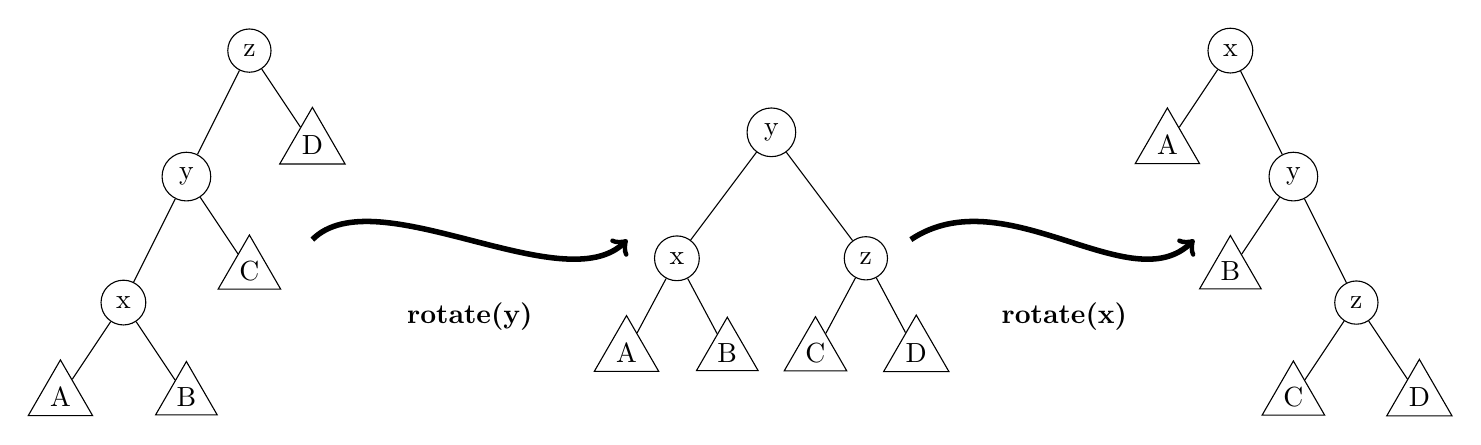
\begin{tikzpicture}[nodes=draw,shape=circle,scale=0.8]
\tikzstyle{subtree}=[regular polygon,regular polygon sides=3,inner sep=1]
\begin{scope}
\node (x) at (0,0) {x};
\node (y) at (1,2) {y};
\node (z) at (2,4) {z};
\node[subtree] (A) at (-1, -1.5) {A};
\node[subtree] (B) at (1, -1.5) {B};
\node[subtree] (C) at (2, 0.5) {C};
\node[subtree] (D) at (3, 2.5) {D};
\draw (x)--(y)--(z);
\draw (A) -- (x) -- (B);
\draw (C) -- (y);
\draw (D) -- (z);
\end{scope}
\draw[->,line width=2] (3,1) .. controls (4,2) and (7,0) .. (8,1) node[below=-0.3,midway,draw=none] {\bf rotate(y)};
\draw[->,line width=2] (12.5,1) .. controls (14,2) and (16,0) .. (17,1) node[below=-0.3,midway,draw=none] {\bf rotate(x)};
\begin{scope}[xshift=250,yshift=20]
\node (x) at (0,0) {x};
\node (y) at (1.5,2) {y};
\node (z) at (3,0) {z};
\node[subtree] (A) at (-0.8, -1.5) {A};
\node[subtree] (B) at (0.8, -1.5) {B};
\node[subtree] (C) at (2.2, -1.5) {C};
\node[subtree] (D) at (3.8, -1.5) {D};
\draw (x)--(y)--(z);
\draw (A) -- (x) -- (B);
\draw (D) -- (z) -- (C);
\end{scope}
\begin{scope}[xshift=500]
\node (x) at (0,4) {x};
\node (y) at (1,2) {y};
\node (z) at (2,0) {z};
\node[subtree] (A) at (-1, 2.5) {A};
\node[subtree] (B) at (0, 0.5) {B};
\node[subtree] (C) at (1, -1.5) {C};
\node[subtree] (D) at (3, -1.5) {D};
\draw (x)--(y)--(z);
\draw (A) -- (x);
\draw (B) -- (y);
\draw (D) -- (z) -- (C);
\end{scope}
\end{tikzpicture}
\end{center}
\caption{\label{zig-zig}Zig-zig step in splay operation (Case 2)}
\end{figure}



After the operation we know that $r'(x) = r(z)$. Using the definition of amortization, 
\[\text{amortized cost} = \text{actual cost} + \Delta \Phi\]

The actual cost is just 2 rotations. We also know that since $x,y, z$ are the only ranks that change, then using $r'(x) = r(z)$

\begin{align}
    \nonumber\Delta\Phi &= (r'(x) + r'(y) + r'(z)) - (r(x) + r(y) + r(z))\\
    \nonumber&= r'(y) + r'(z) - r(x) - r(y)\\
    &= r'(x) + r'(z) - 2r(x) \label{eq:star}
\end{align}

where the last step follows due to $r(x) \le r(y), r'(y) \le r'(x)$ due to the parental relationship between $x$ and $y$ before and after the operation.

We try to bound $r(x)+r'(z)$:
\begin{align*}
    \dfrac{r(x) + r'(z)}{2} &= \lg\left(\sqrt{s(x)s'(z)}\right)\\
    &\le \lg\left(\dfrac{s(x)+s'(z)}{2}\right) &\text{by AM-GM}\\
    &\le  \lg\left(\dfrac{s'(x)}{2}\right) = r'(x) - 1
\end{align*}

where the last line follows since $s(x) = w(x) + s(A) + s(B), s'(z) = w(z) + s(C) + s(D)$, and $s'(x) = w(x) + w(y) + w(z) + s(A) + s(C) + s(D) \ge s(x) + s'(z)$.

Therefore, we have that \[r'(z) \le 2r'(x) - r(x) - 2\]
Subsituting into equation (\ref{eq:star}), we get
\[\Delta \Phi = r'(x) + r'(z)-2r(x) \le r'(x) + 2r'(x) - r(x) - 2-2r(x) = 3(r'(x) - r(x) -2\]

and therefore \[\tilde{t}_2 = 2 + 3(r'(x) - r(x)) - 2 = 3(r'(x)-r(x))\]
as desired.
\end{proof}

So we can say splay and query take $O(\lg n)$, since query is simply walking down the tree and a splay. However, insert must be dealt with differently since we increased the potential function. 

\subsection{Analysis of insert(x)}

The amortized cost of insert is $\Delta\Phi$ from inserting $k$ levels down and $O(splay) = O(\log n)$. It suffices to bound $\Delta\Phi$ from the insert by $O(\log n)$ to achieve the desired amortized runtime.

Suppose in order to insert $x$, its parents above it in the BST are $y_1 = x.parent, y_2 = y_1.parent, ... y_k=root$. Then
\begin{align*}
    \Delta\Phi &= \sum_{j=1}^k r'(y_j) - r(y_j)\\
    &= \sum_j \lg\left(\dfrac{s(y_j) + 1}{s(y_j)}\right) &w(x) = 1\\
    &= \lg\left(\pi_j\dfrac{s(y_j)+1}{s(y_j)}\right)\\
    &\le \lg\left[\dfrac{s(y_2)}{s(y_1)}\cdot\dfrac{s(y_3)}{s(y_2)}\cdot ... \cdot \dfrac{s(y_k)+1}{s(y_k)}\right]
    &s(y_j) + 1 \le s(y_{j+1})\\
    &= \lg\left(\dfrac{s(y_k)+1}{s(y_1)}\right)\\
    &\le \lg (s(y_k) + 1) = O(r(y_k)) = O(\lg n)
\end{align*}

as desired.

\subsection{Static Optimality}
We want to be competitive with a BST built for the distribution of queries given, in the case that there are no inserts or deletes (there's a dynamic programming algorithm for constructing this). We claim that if a sequence of queries $\sigma$ is long enough, splay trees achieve a constant within the optimal static BST, which is proven in the original splay tree paper by Tarjan and Sleator\cite{SJ85-SPLAY}.

Formally, given a query sequence $\sigma$ and fixed BST $T$, 
\[C_{splay}(\sigma) \le O(n^2 + C_T(\sigma))\]

and once $|\sigma^2| > n^2$, this implies $C\cdot OPT$. Note that we can achieve $n\log n$, which is better than $n^2$, though we won't prove it here.

\begin{proof}
Suppose $T$ puts node$x$ at the level $\ell_x$ of the tree where $\ell_{root}=0$. Define $w(X) = \dfrac{1}{3^{\ell_x}}$. 

Recall, \begin{align*}
    \sum(\text{amortized costs}) = \sum(\text{actual costs})+\Phi_{final}-\Phi_{init}\\
    \Rightarrow  \sum(\text{actual costs}) = \sum(\text{amortized costs}) + \Phi_{init} - \Phi_{final}
\end{align*}
we will show that $\sum(\text{amortized costs}) = O(OPT)$ and $\Phi_{init} - \Phi_{final} = O(n^2)$, which is sufficient to prove the claim. Here, we relax the condition that $\Phi$ must be positive and zero on the initial data structure, since we account for the difference in potential explicitly.

\textbf{Difference in potential:} Note that $\Phi(S) = \sum_x \lg (s(x))$, and we want to know how big of a magnitude this can get. Well, we know that $\dfrac{1}{3^n} \le w(x) \le 1$, so $s(x) \ge \dfrac{1}{3^n} \Rightarrow \lg(s(x)) \ge -cn$. So we know that \[\sum_x \lg(s(x)) \ge -cn^2\]
for some constant $c$. Addditionally, we know since each $s(x)\le 1$, that 
\[\sum_x\lg(s(x))\le O(n\log n)\]

Thus, the difference in potential is no more than $O(n^2)$.

\textbf{Amortized costs:} Amortized cost of query(x) is $O($amortized cost of splay(x)). It suffices to show that the amoritized cost of splay(x) is the same cost of accessing an item in the perfect BST $T$, which is $\ell_x$. 
\[O(root) - r(x)) = O\left(\lg\left(\dfrac{W}{s(x)}\right)\right)\]
where $W=\sum_z w(z)$. 

We want this amoritized cost to be $O(\ell_x)$. We note that $W\le C$ for some constant $C$, since \[W = \sum_z w(z) = \sum_z \dfrac{1}{3^{\ell_z}} = \sum_{\ell=0}^n\dfrac{1}{3^\ell}\cdot (\#\text{nodes at level }\ell) \le \sum_{\ell}\dfrac{2}{3}^\ell = O(1)\]

We know that $W\ge 1$, so $W=\Theta(1)$. Therefore,
\begin{align*}
    \lg\left(\dfrac{W}{s(x)}\right) &= \Theta(1) - \lg(s(x))\\
    &= \Theta(1) - \lg\left(\dfrac{1}{3^{\ell_x}}\right)\\
    &= \Theta(1+\ell_x)
\end{align*}

so we are done, sinc ethe cost is exactly a constant factor off of $\ell_x$, the cost in the optimal BST.

\end{proof}


\section{Online Algorithms}
Online algorithms are a class of algorithms in which one must make a sequence of irrevocable decisions without knowing the future. However, we want to be competitive the best sequence of decisions in hindsight. 

\begin{definition}
Let $OPT$ be the optimal strategy given omniscience. We say that a strategy$S$ is $r$-competitive if for a sequence of events $\sigma$
\[cost_{S}(\sigma) \le r\cdot cost_{OPT}(\sigma) + O(1)\]
\end{definition}

\subsection{Examples}
\subsubsection{Ski Rental Problem}
Suppose you are on a ski trip, and you let your friends dictate how long your group will continue skiing. Your friends will inform you each morning whether you will continue to ski that day, or leave the resort. You need skis, and there are two options:
\begin{itemize}
    \item rent skis: \$1 per day
    \item buy skis: \$ B, one time payment at any time
\end{itemize}

If you knew ahead of time how many days you wil stay at the resort $n$, your strategy would be to buy the skis on the first day if $n>B$ and rent otherwise. What should your strategy be to minimize your regret?

\textbf{Strategy:}
You rent for $B-1$ days. If by the $B$th day you did not leave, buy the skis.

This is optimal for staying $\le B-1$ days, and the worst case is if you stay for exactly $B$ days and leave the next day. Then you spent \$2B-1 dollars, but opt spent $B$, so you're always guaranteed to be within a factor of $2$ from the optimal.

Indeed, the ski rental problem has competitve ratio $r=2$, and no other online strategy can do better, which makes it the optimal.

\subsubsection{Free Swag at the Career Fair}
You're standing in the middle of a hallway lined with $2n+1$ rooms at the career fair. Your friend texts you saying that there is some room in which a free laptops (!!!) are being given out by some company who really wants you to work for them. You want to get there as soon as possible, because if you get there too late, all the laptops may be claimed. Walking by a room takes constant time, and looking in as you walk past a room costs no time. What should be your strategy of exploring rooms?

If you knew which room $t$ had the swag in it, you would just walk to $t$, incurring $|t|$ cost to get there.

Suppose you're at room 0, and there are $n$ rooms on either side of you, which we'll number $1,2,...n$ on your right and $-n , -n+1, ... -1$ on your left. One strategy might be to go to rooms $1, -1, 2, -2, 4, -4, ...$ until you find the room that you're looking for. This cost will be 
\[(1+1+1+1) + (2+2+2+2) + (4+4+4+4) + ... = 4(2^0+2^1+...+2^j) \approx 4\cdot 2^{j+1}\]

The worst case scenario arises when the jackpot room is $t=-2^j-1$. Then we would pay $4\cdot 2^{j+1}+2\cdot 2\cdot 2^{j+1} + t = 13t$. So this algorithm is $13$-competitive. 

There exists a 9-competitive strategy where we traverse the rooms $1, -2, 4, -8, ...$, which we won't analyze here. 

\section{List Update Problem}
This mechanism was originally posed by Sleater and Tarjan\cite{SJ85}, before which analysis of this kind was usually done assuming a known distribution of list accesses. 

There are $n$ nodes in a linked list. We are given an access sequence $\sigma$ where $\sigma_i\in [n]$, and we will call query on each of them.

\textbf{query(x):}
\begin{itemize}
    \item start at head of the linked list
    \item cost(query(x)) = depth of $x$ in the linked list
    \item for free, we can move $x$ towards the front of the linked list
    \item for cost $1$, we can swap two adjacent items that are not $x$. 
\end{itemize}

Note that we can view paging as a list update problem with a different cost function, where \[\text{cost(query}(x)) = \begin{cases}0 &\text{if } x\in \text{ first $k$ positions} \\ 1 & \text{otherwise}\end{cases}\]

to simulate having $k<n$ space in cache, and unbounded memory.

\subsection{Different Heuristics}
\begin{itemize}
    \item \textbf{Move to Front:} move $x$ to the front of the list after querying $x$ (note, this is exactly the Least Recently Used cache eviction strategy in paging)
    \item \textbf{Transpose:} move $x$ one position closer to front
    \item \textbf{Frequency count:} Keeps items stored in decreasing order of access frequency
\end{itemize}

\bibliographystyle{alpha}

\begin{thebibliography}{42}

\bibitem{SJ85}
Daniel~Dominic~Sleator, Robert~Endre~Tarjan.
\newblock Amortized Efficiency of List Update and Paging Rules.
\newblock {\em Communications of the ACM}, 28(2):202--208, 1985.

\bibitem{SJ85-SPLAY}
Daniel~Dominic~Sleator, Robert~Endre~Tarjan.
\newblock Self-adjusting binary search trees. 
\newblock {\em J. ACM},
32(3):652–686, 1985.

\end{thebibliography}

\end{document}